\documentclass[12pt]{article}
\usepackage{url}
\usepackage[a4paper, total={6in, 8in}]{geometry}
\usepackage{hyperref}
\usepackage{titlesec}
\usepackage{graphicx}
\usepackage{amsmath}
\setcounter{secnumdepth}{4}

\titleformat{\paragraph}
{\normalfont\normalsize\bfseries}{\theparagraph}{1em}{}
\titlespacing*{\paragraph}
{0pt}{3.25ex plus 1ex minus .2ex}{1.5ex plus .2ex}

\begin{document}

\title{WikiGaze: Wikipedia Analyzes through Gaze Based Personalized Summaries}
\maketitle

\begin{abstract}
  Due to it's complex collaborative structure and huge success, Wikipedia has been vastly analyzed from various perspectives. 
As a result, now we decently understand the overall nature of Wikipedia editors' collaboration dynamics and various features of it's articles. 
But a little research has been performed to understand readers' perspective about Wikipedia. 
In this paper, we propose a novel approach to analyze how a reader refers Wikipedia articles. 
This is attained by capturing the reading pattern of readers. 
We implement a state-of-the-art method to generate personalized summaries of Wikipedia articles through eye gaze tracking of a reader. 
These summaries capture reader's attention pattern. 
Summaries thus generated are gathered and analyzed for evaluation of different features of Wikipedia from readers' perspective. 
Using the proposed method, we develop a cross-platfrom document summarization and analysis tool. 
The experimental results show the efficiency of our personalized summary generation approach and the proposed analysis method of Wikipedia articles also show some interesting results.
\end{abstract}


\section{Introduction}
Wikipedia grows constantly as new entries are being continuously added by users throughout the world. This open-content encyclopedia is a unique and aptly named reference resource. It allows for public authorship and editing of any of its articles. Post its inception in 2001, Wikipedia has seen exponential growth. Currently, it posses more than 48 million pages and 37 million contributors in the English Wikipedia alone~\cite{wiki:Wikipedia:Statistics}. It has been consistently ranked in the top ten visited sites on the Internet as per Alexa.com. Past studies show that Wikipedia's content quality is comparable to traditional encyclopedias~\cite{giles2005internet}. Search engines such as Google and Bing respond to user queries by extracting structured knowledge from Wikipedia~\cite{bergstrom2009conversation}.


The users of Wikipedia can be divided into two sets; the production team members(editors, moderators) and the passive team members(readers). Most of the researches performed to analyze various characteristics of Wikipedia revolve around understanding the behavior of the production teams, i.e. editors, moderators and their collaboration dynamics. A study~\cite{okoli2012people} performed on 477 Wikipedia based researches revealed that 42\% of these reseachers were centered on understanding characteristics of contributors involment or article quality evaluation~\cite{wilkinson2007assessing, kittur2008harnessing, stvilia2008information}. Only 20\% of the studies related to readers in Wikipedia and the usage of Wikipedia. Less than 1\% of the reviewed studies looked at users' reading preferences.
%and only one study investigated reading behavior~\cite{okoli2012people}. 
%performed by Okoli et al.


The study by Antin et al.~\cite{antin2010readers} claims that reading can be seen as a form of participation and is therefore valuable. Reading a Wikipedia article can be considered as a legitimate peripheral participation through which individuals gain knowledge and can move towards more active participation. The fact that a user is reading an article and not editing could be interpreted as an indication of an article's quality, such as its reliability~\cite{adler2008assigning}. Thus, focus on reading activity can provide valuable insights to the article evaluation. Lehmann et al.~\cite{lehmann2014reader} emphasized on the importance of reading behavior analyses. The research characterizes users' reading preferences at article level i.e. it determines which articles are more ``engaging" than others. 


In order to perform detailed analyzes like, evaluation of a reader's attention span distribution over an article or understanding the readability issues within an article; we need to capture a reader's perception of the article. By tracking the reader's interest pattern over an article a granular analyzes can be performed. In past studies~\cite{calder2002reading, bff9c00ddce3404ca729f4a96d53a701}, it was revealed that our eye gaze pattern is closely related to our thought process. Through eye gaze tracking, we can get the knowledge about the portions of an article where a user is more focused while reading. There is evidence in research from reading psychology that eye movement patterns while reading are indeed related to textual features~\cite{rayner1978eye}.


To analyze Wikipedia articles on content level, we need a dataset containing gaze information of several users who have read a particular article. Generating such dataset requires a technique which is easy to use and available at users' site. 


\subsection{Our Contribution}
In this paper, we propose a novel approach to capture reading pattern of Wikipedia users. Using a simple \emph{web camera} and some computer vision technique, we track the eye gaze pattern of a user while he is reading an article. Based on his ``gaze heat map" we extract the portions of the article where he was more focused while reading and create a personalized summary for him. User is also allowed to provide his requirement for the length of the summary. According to the length requirement we decide the threshold to perform text extraction from the article. 


For a particular article, multiple users generate their personalized summaries. We ask the users to share their summaries for analyzes purpose.  Due to privacy reasons, some users might not be willing to share their data. As an incentive mechanism we implement a special feature to generate ``recommended summary". To unlock this feature, a user must share their data with the central analyzes team. Each user is given a special ID to maintain anonymity. We develop a cross-platform standalone application to generate personalized summary and to recommend summaries based on user's past reads. 


We gather shared summaries and gaze heat-map of each user for various articles to produce a benchmark dataset. This dataset contains the reading pattern of Wikipedia users. To the best of our knowledge, no such dataset exists.


On the dataset thus collected, various analyzes results can be produced. In this paper we show two such analyzes. The first analyzes prepares a leader-board for Wikipedia editors based on their content contribution presence in various summaries. This leader-board is prepared on article level. The rational behind this analyzes is to judge editors' contribution based on the extent to which it is being read by other users. In second analyzes we try to find the correlation between summary length and article length. This is to analyze if users get discouraged by long article and read less or the length of an article does not effect the reading extent. We discuss analyzes results in later sections.  



The key contribution of our work is as follows:
\begin{itemize}
	\item A state-of-the-art approach to generate personalized summaries based on eye gaze tracking.
	\item A novel approach to analyze Wikipedia articles based on users' reading pattern.
	\item Development of a cross-platform application to generate personalized summaries and recommend summaries.	
\end{itemize}



\subsection{Paper Structure}
The structure of rest of the paper is as follows. \hyperref[sec:Related]{Section 2} points on some of the related works. \hyperref[sec:Proposed]{Section 3} explains the proposed Wikipedia analyzes technique. In \hyperref[sec:Analysis]{Section 4} we explain how the proposed technique can be utilized to analyze Wikipedia articles. \hyperref[sec:Resources]{Section 5} explains the online resources provided. \hyperref[sec:Discussion]{Section 6} contains a detailed discussion on the proposed method. \hyperref[sec:Conclusion]{Section 7} concludes and discusses future work.


\section{Background \& Related Work}\label{sec:Related}

On abstract level, research on Wikipedia can be divided into two classes: one that \emph{studies} Wikipedia and other that \emph{uses} Wikipedia as a source of knowledge.


\subsection{Relation between Eye Gaze and Reading Pattern}
Eye movement characteristic of reading is extensively studied in the psychology literature~\cite{rayner1998eye}. Eye movement tracking open the door for an automated analysis of document reading. 

In~\cite{beymer2005webgazeanalyzer} a system is proposed for recording and analyzing web reading behavior using eye gaze.

Sanches et. al~\cite{sanches2018estimation} show that prediction of the subjective understanding is improved by 13\% if we use eye gaze instead of comprehension questions.


\subsection{Personalized Summarization Techniques}
    
    
    
\subsection{Wikipedia Analysis Techniques}
There have also been quantitative studies that attempt to assess the
quality of Wikipedia articles in a more objective way using metrics based on the meta-data associated with Wikipedia itself. Blumenstock simply uses the word count of an article as a measure of
quality [2]. Lih [14] has suggested the number of edits and unique
contributors of an article as measure for quality, where the number
of unique authors reveals the “diversity” of an article and the number of edits its “rigor”. Wilkinson et al. have demonstrated later
that high-quality vs. non-featured articles have indeed substantially
more contributors involved [25]. In [1], these two measures are
combined to define the notion of “author reputation”. Other single metrics based on the agregation of several indicators have been
proposed to predict the quality of a contribution [7] or the trustworthiness of an article [6]. In addition the collaborative work in
dedicated “discussion pages” — where changes are often discussed
before being introduced in the article [21] — plays a critical role in
the quality of articles [11, 23].
A common trend in these studies is that the metrics reveal social
information that can be used as an indicator for assessing the quality of an article. It has been shown that revealing trust-relevant
information to the users has an effect on the trustworthiness of the
articles [12, 15], and three visual tools have been proposed aiming
at enhancing the user and reader experience on Wikipedia.



\section{Proposed Method}\label{sec:Proposed}

Cross-platform application (Ubuntu, Mac, Windows)...Application detail...\\
1: Summarization (basic feature...)\\
2: Summary recommendation (advanced feature...)


We present a novel approach to analyze Wikipedia articles by capturing the reading pattern of users, through personalized summaries. 

\subsection{Personalized Summarization}

Document summarization reflects the key points of the document which the summarizer tool deems important. The summary thus produced is generic in nature. In many situations, users are interested in facts more relevant to them; motivating the need for query-relevant or personalized summaries. For instance, consider a sports enthusiast who wants to know about the sports culture in United States by reading its' Wikipedia article. A more useful summary for this person would contain sports related passages assembled into a short document. We can say that users with different information needs require different summaries of the same document.

Personalization has been identified as being one of the grand challenges in information retrieval lately~\cite{belkin2008some}. Personalized summarization~\cite{berkovsky2008aspect} presents users with document extracts that are of interest to them. Manual filtering of information from large documents is a tiresome task. Therefore it becomes extremely significant to automate this process. Majority of the automatic personalized summarization techniques incorporate some kind of personal information for individually improving the quality of summary~\cite{moro2012personalized, wu2008personalized, kumar2008generating}. The proposed technique does not require the users to share any personal information. 


Spacial and temporal gaze patterns are valuable pieces of information and can be used to infer present cognitive processes of the user \cite{Beymer:2005:WSC:1056808.1057055}. We utilize the eye gaze pattern to extract more focused portions of the text and assemble them to generate personalized summary. In following subsections, we address methods and measures to generate a summary.

\subsubsection{Eye Gaze Tracking}
Eye gaze tracking is the process to estimate the direction of gaze and the point of regard. Rayner~\cite{rayner1998eye} provides a comprehensive overview of the studies concerning gaze pattern while reading. The eye shows a characteristic behavior composed of a series of fixations and saccades. Fixation is a duration for which the eye is steadily gazing at one point. On average it is of time interval 200-250 ms. Saccade is a rapid eye movement from one fixation to the next. For languages written left-to-right; approximately 10-15\% of the eye movements during reading are regressions, i.e., movements to the left along the currently focused line. A regression, or backwards eye movement in the text, is a sign that the
reader is having difficulty understanding the material.

Well established devices, like Tobii~\cite{olsen2012tobii}, EyeLink~\cite{cornelissen2002eyelink}, etc. are available for gaze tracking. Though they provide higher accuracy, they are quite expensive and rarely available at user's site. Applying eye tracking to reading analysis requires a basic trade off between the invasiveness of the eye tracker and the accuracy of the estimated gaze points. To collect the dataset of Wikipedia reader's gaze pattern, we require a feasible, easy to use solution. 
Therefore we obtain gaze samples through vision-based commodity eye tracking. We assemble an eye-tracking setup containing a Logitech Webcam C922 Pro Stream and readily available eye-tracker applications. Table 1 shows the details of the eye-trackers used for various platforms. 
The main reason behind selecting these trackers is to make our tool platform independent. CVC ET~\cite{ferhat2014cheap, CVC} is the port of Opengazer for the Linux and Mac platform and NetGazer~\cite{WinNT} is the port of Opengazer for the Windows platform. CVC ET as well as NetGazer are open-source softwares. The CVC ET is actively maintained by researchers from Universitat Aut\'{o}noma de Barcelona~\cite{CVC}. It provides 1.47$^{\circ}$ horizontal error and 1.35$^{\circ}$ vertical error. NetGazer is not maintained anymore therefore we updated the package based on CVC ET functions; since they both are based on Opengazer project. 

\begin{table}[]
\begin{tabular}{|c|c|c|c|c|c|c|}
\hline
Tool     & Language & Platform  & Vertical Error & Horizontal Error & License & Reference                     \\ \hline
NetGazer & C++/C\#  & Windows   & 1.55$^{\circ}$ & 1.62$^{\circ}$   & GPLv2   & \cite{WinNT} \\ \hline
CVC ET   & C/C++    & Linux/Mac & 1.35$^{\circ}$ & 1.47$^{\circ}$   & GPLv2   & \cite{CVC}   \\ \hline
\end{tabular}
\caption{Detail of eye-trackers used for various platforms.}
\label{tab:eye_tracker}
\end{table}

To meet our requirement we modified some of the functions of the eye-trackers. The assembled setup containing a simple camera and the selected eye-trackers, is non-invasive, cost effective and platform independent. 


Using Webcam, we record reader's facial video and feed this as input to the eye-tracker. Eye tracker detects eye gaze direction in the video and maps the gaze to the location on the screen where the user is looking at. 


Mathematical formula for gaze mapping on screen...

This process continues during the entire reading session. The time-series data of on-screen gaze locations are captured. 



\subsubsection{Wikipedia Specific Text Extraction}

Ajanki et.al~\cite{bff9c00ddce3404ca729f4a96d53a701} claim that when the system has no prior information as to what the user is searching, the eye movements help significantly in the search. This is the case in a proactive search, for instance, where the system monitors the reading behaviour of the user in a new document. Xu et al.~\cite{xu2009user} talk about the relevance between the human text reading pattern and their current cognitive process. Their basic assumption is that the eyes' fixation duration on a word is directly equivalent to the user's interest in that word. 


%%CHANGE%%
First, our reading analysis deals
with inherent noise and drift problems in remote trackers –
fixations are grouped along horizontal scans and matched
against the text DOM lines in a robust manner. While
mapping a single fixation to the text lines may be
ambiguous, the matching of groups of fixations to chunks
of the DOM can resolve this ambiguity. 
%%CHANGE%%

Based on these assumptions we create a sentence ranking mechanism based on the duration for which it was being gazed by a user.

equation to identify the "selected area" for text extraction.

Generate heat map using:
Identify the thresholded contours on the image:
Extract the text from image:

Based on heat-map we extract text from images. Bounding box formation : wiki specific
        
        
\subsubsection{Summarization}
%We have implemented two layers of summarization..


The main goal of extractive summarization can be
concisely formulated as extracting from the input
pieces of text which contain the information about
the most important concepts mentioned in the input
text or texts. This definition conceals a lot of important issues that should be taken into consideration
in the process of summary construction

what does it depict?


%\paragraph{Abstractive Summarization}
%abstractive summarization systems generate new phrases, possibly rephrasing or using words that were not in the original text


\subsection{Summary Recommendation System}
%%%%%%%change%%%%%%%%
    One possibility is that having many
contributors results in higher quality and less biased articles.
The benefits of aggregating judgments from many people
have been observed since at least 1907, when Galton showed
that averaging independent judgments of many observers
estimated the weight of an ox at a county fair better than
experts could [7]. The Internet makes aggregating
judgments much easier, leading to systems of collective
intelligence ranging from markets for accurately predicting
presidential elections [3] to systems where volunteers
classify craters on Mars' surface, resulting in work virtually
indistinguishable from that of expert geologists [17]. Most
models of collective intelligence are premised on
aggregating the independent contributions of many people,
colloquially known as harnessing ``the wisdom of crowds" [32]
%%%%%%%change%%%%%%%%


Paper on recommending personalized summary \cite{cagliero2019recommending}

\section{Wikipedia Analysis}\label{sec:Analysis}
Based on the summary created, we can capture the article reading pattern. This can serve as a novel dimension to analyze Wikipedia articles. 

    
\subsection{Editor's Contribution Analysis}
Wikipedia is a crowd-sourced online community for knowledge building. A characteristic feature of such online communities and social media sites is the mechanism for rewarding user achievements. It is primarily done to motivate users to enhance their on-site participation. There exists a strong correlation between editor contribute and article quality~\cite{li2015automatically}. 
Leaderboards are commonly used by participants to compare their performance against others and reward them by publically enhancing their rank. Blum et. al~\cite{blum2015ladder} show the importance of leaderboard creation and how participants' ranking affects their future performance.

Each editor in Wikipedia contributes some facts to the article. Therefore a naive way to rank editors' contribution is by comparing their individual contributions in bytes. This method has several prominent disadvantages, like the quality of the contribution will not be captured this way. An editor who adds much random text in the article can be ranked higher than an editor who contributes 2-3 relevant sentences. There have been several attempts to understand the collaboration dynamics of Wikipedia editors~\cite{kim2016understanding, sepehri2012leveraging, wagner2016women}. These studies evaluate the performance of production side users, like, editors from the article content production perspective alone. 

In the proposed evaluation technique we bring in the perspective of passive side users, i.e., readers. This will enable capturing the perception of editors content contribution by it's readers. An editor who's contribution is more referred by readers can be assumed to have a better understanding of the readers requirement and therefore should be given higher preference in leaderboard. Using the personalized summaries gathered for an article, we create a model to rank it's editors contribution. 

Given a personalized summary, we create a list of all the editors whose content appear in this summary. This list is created by tracing back along the article revision history to search which editor first added that particular content. We sort this list as per editor's contribution bytes present in the summary and rank the editors. Editors rank is zero if his contribution is not present in a summary. For all the summaries of a particular article this process is repeated. Each editor is given a score which is a function of editors rank in a summary and the number of bytes of his contribution content in the summary.   



\begin{figure}[!htb]
        \center{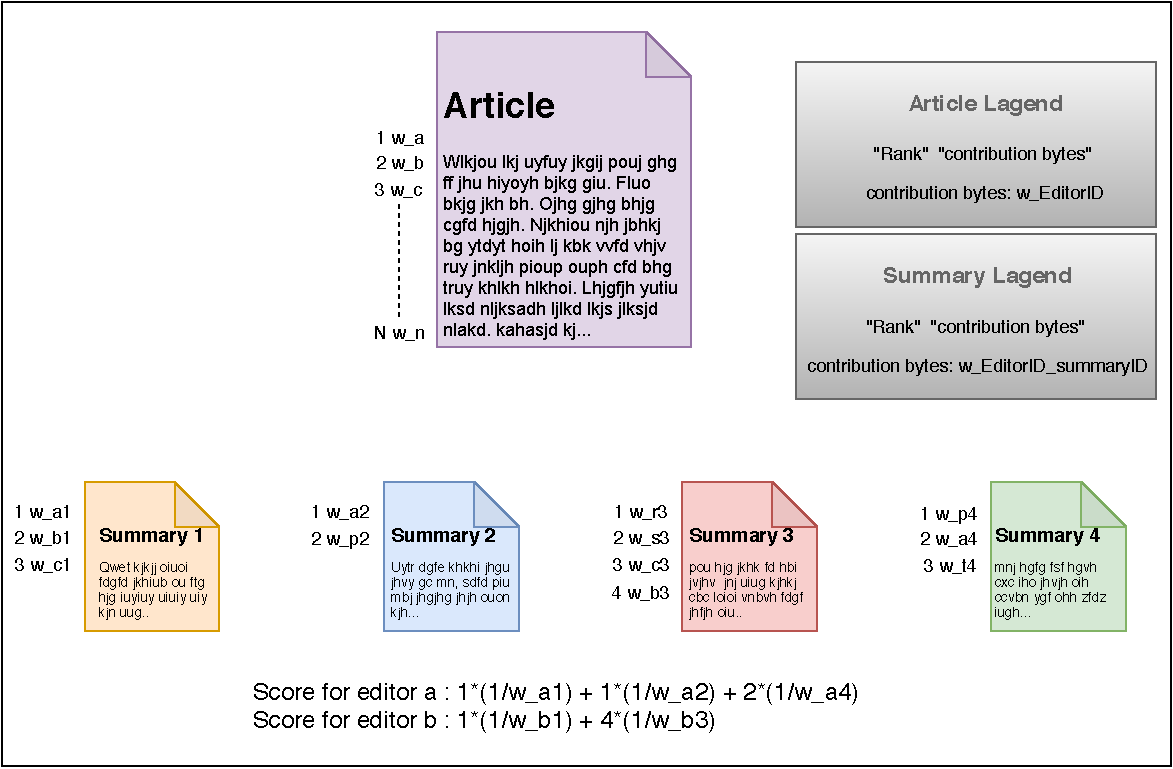
\includegraphics[width=\textwidth]
        {images/editor_contrib.pdf}}
        \caption{\label{fig:editor_contrib} Formula to calculate editor score}
\end{figure}

General formula to calculate editor ($x$) score:
\begin{equation}
	Score_x = \sum_{k=0}^{k=m}I_x(k)\begin{bmatrix}R_x(k).\frac{1}{w\_xk}\end{bmatrix}
\end{equation}
    where, $m$ is the number of summaries of article under consideration. $I_x(k)$ is an indicator function. 
If $I_x(k)=1$, it implies that summary $k$ contains content contributed by editor $x$ and 0 otherwise.
$R_x(k)$ refers to the rank of editor $x$ in summary $k$ and $w\_xk$ refers to the number bytes present in the summary $k$ which was contributed by editor $x$.

The lower the score, the better the rank of an editor on leaderboard. The score is directly proportional to the rank of an editor in a summary and inversely proportional to the contribution bytes in that summary. This is done to nullify the impact of varying summary lengths.



Table of analyzes for editor ranking in an article and our ranking.


    
%\subsection{Relation between Summary Length \& Article Length}
\subsection{Relation between Article Length and it's Reading Extent}    
Article length is considered an effective metric for analysing an article~\cite{chevalier2010wikipediaviz, dang2016quality}.   Falagas et. al~\cite{falagas2013impact} demonstrates the impact of article length on the number of citations that it might get in future. Blumerstock ~\cite{blumenstock2008size} shows that article length is a critical parameter  to differentiate featured articles from other articles in Wikipedia. 
But it can not be said that all long articles are good.~\cite{blumenstock2008size} shows several counterexamples that prevent using it alone as a quality measure.

While article length plays an important role in analyzing an article from various aspects, does it actually motivate a reader to read the article more or it discourages the reader to read it completely. Readers can be considered as clients for a Wikipedia article. Therefore it becomes essential to analyze the correlation between the length of an article and the extent to which it is read by users.

To determine the relationship between article length and it's reading extent
we need a mechanism to capture how much an article is read by a user. This is facilitated by the personalized summary that we create by analyzing user's reading pattern. Summary demonstrates the portion of the article which was read with focus. Therefore, we can use the summary length to measure the reading extent of an article.



plot of different summary lengths of an article (long article \& short article)

plot of article length and average summary length



Conclusions....

    
    
\subsection{Relation between Gaze Pattern and Article Readability}    
Automating the process of measuring the quality of a Wikipedia article has been an important task since last ...... Several attempts have been made in this regard....
cite....
cite....
cite....

All these approaches require devising a complex feature set or using some machine learning approach to quantify the quality of an article. 

In the porposed approach we try to find out the relationship between article quality and gaze pattern.

Samples grid...

Features of gaze heatmap to evaluate article quality...

plot for these features...

Conclusions...
    
\section{Online Resources}\label{sec:Resources}


\section{Discussion}\label{sec:Discussion}


\section{Conclusion \& Future Work}\label{sec:Conclusion}

\newpage

\bibliography{neeru} 
\bibliographystyle{ieeetr}

\appendix

\section{Research Methods}

\subsection{Part One}



\subsection{Part Two}


\section{Online Resources}




\end{document}
